\section{S/W Block Diagram}
\label{section_SWBD}

In the S/W Block Diagrams for emitter (Figure \ref{fig:SWBDemit} on page \pageref{fig:SWBDemit}) and receiver (Figure \ref{fig:SWBDrec} on page \pageref{SWBDrec})  it could be seen how the different software modules interact with the output interfaces (represented by a circle) and the input interfaces (represented by a rhombus) of various devices on the satellite. 
 
Since the detailed implementation of the satellite software is outside of the scope of this feasibility, the modules and interactions depicted are somewhat abstract.  

From the Block Diagram it could be seen that Attitude \& Sun Position Processing Module is responsible for obtaining information from \ac{ADS} and pointing the satellite and solar panels in the appropriate direction. It works along with Receiver Pointing Determination Module to determine where to point the receiver. Power Calculation Model determines whether to recharge or to use batteries based on the available solar power. Data storage is used to store all the data from various sensors for housekeeping purposes. Photon-Location-Time Registration module registers position and time when a photon is received to Data Storage.

\begin{landscape}
\begin{figure}[ht!]
\centering
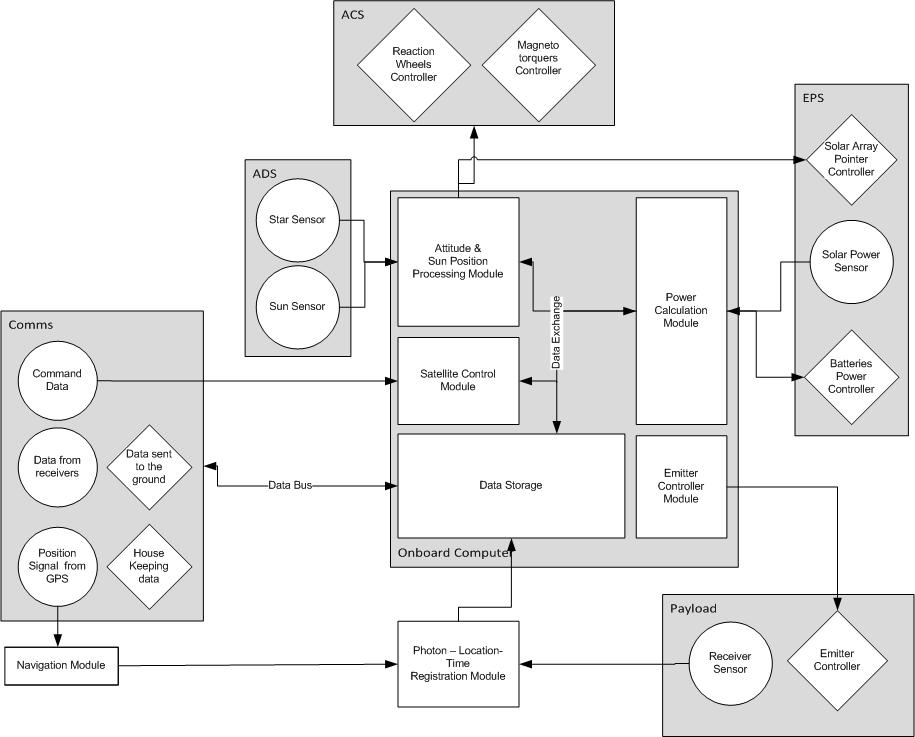
\includegraphics[width=1.3\textheight]{chapters/img/SWBDemit.jpg}
\caption{S/W Block Diagram for Emitter }
\label{SWBDemit}
\end{figure}
\end{landscape}

\begin{landscape}
\begin{figure}[ht!]
\centering
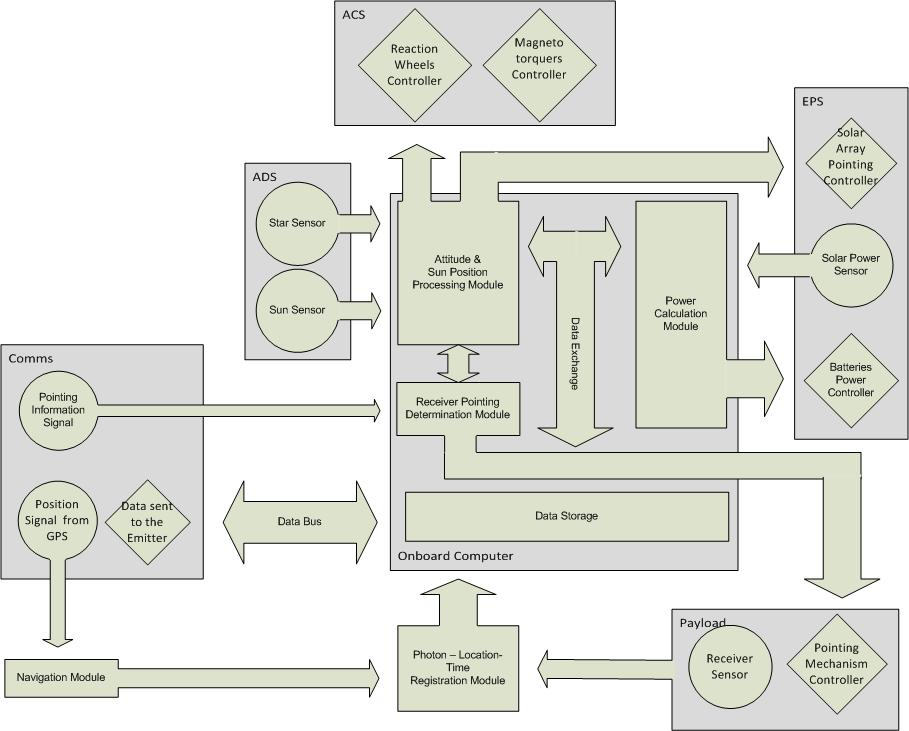
\includegraphics[width=1.3\textheight]{chapters/img/SWBDrec.jpg}
\caption{S/W Block Diagram for Receiver}
\label{SWBDrec}
\end{figure}
\end{landscape}